\documentclass{bioinfo}
%DIF LATEXDIFF DIFFERENCE FILE
%DIF DEL phylotyper.tex           Mon Apr 10 13:54:30 2017
%DIF ADD phylotyper_revised.tex   Fri Jun  2 15:22:46 2017
\copyrightyear{2017} \pubyear{2017}

\access{Advance Access Publication Date: Day Month Year}
\appnotes{Application Note}

\usepackage{url}
%DIF PREAMBLE EXTENSION ADDED BY LATEXDIFF
%DIF UNDERLINE PREAMBLE %DIF PREAMBLE
\RequirePackage[normalem]{ulem} %DIF PREAMBLE
\RequirePackage{color}\definecolor{RED}{rgb}{1,0,0}\definecolor{BLUE}{rgb}{0,0,1} %DIF PREAMBLE
\providecommand{\DIFadd}[1]{{\protect\color{red}#1}} %DIF PREAMBLE
\providecommand{\DIFdel}[1]{{\protect\color{red}\sout{#1}}}                      %DIF PREAMBLE
%DIF SAFE PREAMBLE %DIF PREAMBLE
\providecommand{\DIFaddbegin}{} %DIF PREAMBLE
\providecommand{\DIFaddend}{} %DIF PREAMBLE
\providecommand{\DIFdelbegin}{} %DIF PREAMBLE
\providecommand{\DIFdelend}{} %DIF PREAMBLE
%DIF FLOATSAFE PREAMBLE %DIF PREAMBLE
\providecommand{\DIFaddFL}[1]{\DIFadd{#1}} %DIF PREAMBLE
\providecommand{\DIFdelFL}[1]{\DIFdel{#1}} %DIF PREAMBLE
\providecommand{\DIFaddbeginFL}{} %DIF PREAMBLE
\providecommand{\DIFaddendFL}{} %DIF PREAMBLE
\providecommand{\DIFdelbeginFL}{} %DIF PREAMBLE
\providecommand{\DIFdelendFL}{} %DIF PREAMBLE
%DIF END PREAMBLE EXTENSION ADDED BY LATEXDIFF

\begin{document}
\firstpage{1}

\subtitle{Subject Section}

\title[short Title]{Phylotyper: {\it In silico} predictor of \DIFdelbegin \DIFdel{molecular }\DIFdelend subtypes from gene sequences}
\author[Whiteside \textit{et~al}.]{Matthew D. Whiteside\,$^{\text{\sfb 1,}*}$, Chad R. Laing\,$^{\text{\sfb 1}}$ and Victor P.J. Gannon\,$^{\text{\sfb 1,}*}$}
\address{$^{\text{\sf 1}}$National Microbiology Laboratory, Public Health Agency of Canada, Lethbridge, AB, Canada, T1J 3Z4}

\corresp{$^\ast$To whom correspondence should be addressed.}

\history{Received on XXXXX; revised on XXXXX; accepted on XXXXX}

\editor{Associate Editor: XXXXXXX}

\DIFdelbegin %DIFDELCMD < \abstract{\textbf{Summary:} Whole genome sequencing (WGS) is being adopted in public health for improved surveillance and outbreak analysis.
%DIFDELCMD < Molecular subtyping has been used in public health to infer phenotypes and flag high-risk bacterial strain groups.
%DIFDELCMD < \textit{In silico} tools that predict molecular subtypes from gene sequences are needed to transition historical data to WGS-based protocols.
%DIFDELCMD < Phylotyper is a novel solution for \textit{in silico} molecular subtype prediction from gene sequences.
%DIFDELCMD < Designed for incorporation into WGS pipelines, it is a general prediction tool that can be applied to most molecular subtype schemes.
%DIFDELCMD < Phylotyper uses phylogeny to model the evolution of the subtype and infer subtypes for unannotated sequences.
%DIFDELCMD < The phylogenic framework in Phylotyper improves accuracy, provides useful contextual feedback, and is more capable of identifying novel subtypes over approaches based solely on sequence similarity.\\
%DIFDELCMD < \textbf{Availability and Implementation:} Phylotyper is a python package. It is available from: \url{https://github.com/superphy/insilico-subtyping}.\\
%DIFDELCMD < \textbf{Contact:} \href{matthew.whiteside@phac-aspc.gc.ca}{matthew.whiteside@phac-aspc.gc.ca}\\
%DIFDELCMD < \textbf{Supplementary information:} Supplementary data are available at \textit{Bioinformatics}
%DIFDELCMD < online.}
%DIFDELCMD < %%%
\DIFdelend \DIFaddbegin \abstract{\textbf{Summary:} Whole genome sequencing (WGS) is being adopted in public health for improved surveillance and outbreak analysis.
In public health, subtyping has been used to infer phenotypes and distinguish bacterial strain groups.
\textit{In silico} tools that predict subtypes from sequences data are needed to transition historical data to WGS-based protocols.
Phylotyper is a novel solution for \textit{in silico} subtype prediction from gene sequences.
Designed for incorporation into WGS pipelines, it is a general prediction tool that can be applied to different subtype schemes.
Phylotyper uses phylogeny to model the evolution of the subtype and infer subtypes for unannotated sequences.
The phylogenic framework in Phylotyper improves accuracy over approaches based solely on sequence similarity and provides useful contextual feedback.\\
\textbf{Availability and Implementation:} Phylotyper is a python and R package. It is available from: \url{https://github.com/superphy/insilico-subtyping}.\\
\textbf{Contact:} \href{matthew.whiteside@phac-aspc.gc.ca}{matthew.whiteside@phac-aspc.gc.ca}\\
\textbf{Supplementary information:} Supplementary data are available at \textit{Bioinformatics}
online.}
\DIFaddend 

\maketitle

\section{Introduction}

Whole-genome sequencing (WGS) is transforming the public health field by providing an efficient method for surveying bacterial populations.
The speed, discriminatory power and broad utility of WGS can improve surveillance and outbreak analysis.
Adoption of WGS in public health, however, requires transitioning of historical data with the new methods \citep{Jenkins2015}.
One of the workhorse methods in public health is \DIFdelbegin \DIFdel{molecular subtyping(such as serotyping)}\DIFdelend \DIFaddbegin \DIFadd{subtyping.
Subtyping methods can broadly be categorized as phenotype-based or DNA-based.
Phenotype-based subtypes are, for example, interrogated by biochemical tests (biotyping), detection of surface antigens (serotyping) or susceptibility to bacteriophage (phagetyping) \mbox{%DIFAUXCMD
\citep{Wiedmann2002}
}%DIFAUXCMD
.
Alternatively, DNA-based subtyping examines and classifies bacteria based on genetic content.
DNA-based subtypes use a variety of methods from PCR to Pulse Field Gel Electrophoresis to DNA sequencing to assign groups to bacteria \mbox{%DIFAUXCMD
\citep{Wiedmann2002}
}%DIFAUXCMD
}\DIFaddend .
As a surveillance tool, subtypes provide a \DIFdelbegin \DIFdel{clearcut }\DIFdelend \DIFaddbegin \DIFadd{clear cut }\DIFaddend designation that is typically used to distinguish taxonomic groups and infer phenotypes\DIFdelbegin \DIFdel{, for example, pathogens from non-pathogens}\DIFdelend .
A WGS-based approach to subtyping would have several benefits over current subtype systems; it would be faster, have improved discrimination and would be cheaper and easier to maintain\citep{Jenkins2015}.
Accordingly, new \textit{in silico} tools have been developed to predict subtypes from WGS data \citep{Joensen2015,Ingle2016,CARRILLO2016}.
\DIFaddbegin \DIFadd{To predict from WGS data, these tools have targeted subtypes (either Phenotype-based or DNA-based systems) that can be predicted by sequence variation in a specific region or gene in the genome.
}\textit{\DIFadd{In silico}} \DIFadd{subtype prediction is not applied to subtyping methods that already directly use the DNA sequence to assign subtype such as Multi-Locus Sequence Typing (MLST). 
No inference or extrapolation is needed to integrate a direct DNA sequence-based method, like MLST, into a WGS system.
An example of a subtyping system that has been adapted for WGS is serotyping in }\textit{\DIFadd{Escherichia coli}}\DIFadd{.
The sequence of O-antigen processing genes in }\textit{\DIFadd{E. coli}} \DIFadd{is used to predict O-antigen group serotype in \mbox{%DIFAUXCMD
\citep{Joensen2015,Ingle2016}
}%DIFAUXCMD
.
Another example is the Shiga toxin subtype (Stx); a DNA-based subtyping scheme generated using PCR.
The tool in \mbox{%DIFAUXCMD
\citep{CARRILLO2016}
}%DIFAUXCMD
predicts Stx subtype by simulating PCR }\textit{\DIFadd{in silico}}\DIFadd{.
}\DIFaddend 

Phylotyper is a novel \textit{in silico} predictor of subtypes from sequence data.
\DIFaddbegin \DIFadd{Similar to \mbox{%DIFAUXCMD
\citep{Joensen2015,Ingle2016,CARRILLO2016}
}%DIFAUXCMD
, it also works on subtypes that can be predicted from specific, pre-selected gene or genomic region sequences.
}\DIFaddend Phylotyper is unique in that it builds a phylogenetic tree consisting of reference sequences with known subtype and the unknown query sequences to help inform subtype prediction.
Using phylogenetic ancestral state reconstruction to assign the likelihood of each subtype to the tree branch points, Phylotyper \DIFaddbegin \DIFadd{then }\DIFaddend assigns an unknown query sequence a subtype based on the extrapolated value from its ancestors in the tree.

\section{Implementation}

The core of Phylotyper is an ancestral state reconstruction (ASR) method that has been adapted for hidden state prediction.
In phylogenetic analysis, ancestral state reconstruction involves the prediction of traits of ancestors from existent descendants.
This methodology can be extended to also predict properties in a limited number of existing strains.

In Phylotyper, the \texttt{rerootingMethod} function from the phytools R package is used to perform the ASR \citep{Revell2011}.
This function calculates the maximum marginal likelihood for unknown tip nodes in a phylogenetic tree.
The likelihood reflects the most likely state for the node given the empirically estimated subtype evolution model and phylogeny.
In the context of Phylotyper, the marginal likelihood provides a confidence value associated with a predicted subtype.

Phylotyper is developed in python and R. 
The steps in the Phylotyper pipeline are: 
(1) Identify subtype gene loci in input genomes using BLAST \citep{Camacho2009}. \DIFaddbegin \DIFadd{Inputs are in fasta format. Hits that do not align over 95}\% \DIFadd{or have under 90}\% \DIFadd{sequence identity with a reference sequence are discarded. Users are notified if no loci are found in genome.
}\DIFaddend (2) Align input genes against a pre-aligned set of reference genes using MAFFT's \texttt{--add} feature \citep{Katoh2013}.
(3) If multiple loci are involved, concatenate individual alignments into superalignment.
(4) Generate maximum likelihood phylogenetic tree of aligned genes with FastTree \citep{Price2010}.
(5) Run phytools \texttt{rerootingMethod} using the phylogenetic tree and assigned subtypes \citep{Revell2011}.
(6) Identify the subtype with maximum marginal likelihood for the unknown genes and report to user in text output file.
Users are also provided with an image of the phylogenetic tree overlaid with the likelihood values (e.g. Figure~1\vphantom{\ref{fig:01}}).

\DIFaddbegin \DIFadd{Detailed descriptions on how to run Phylotyper are provided here: }\url{https://github.com/superphy/insilico-subtyping}\DIFadd{.
}

\DIFaddend \begin{figure}[!tpb]%figure1
\centerline{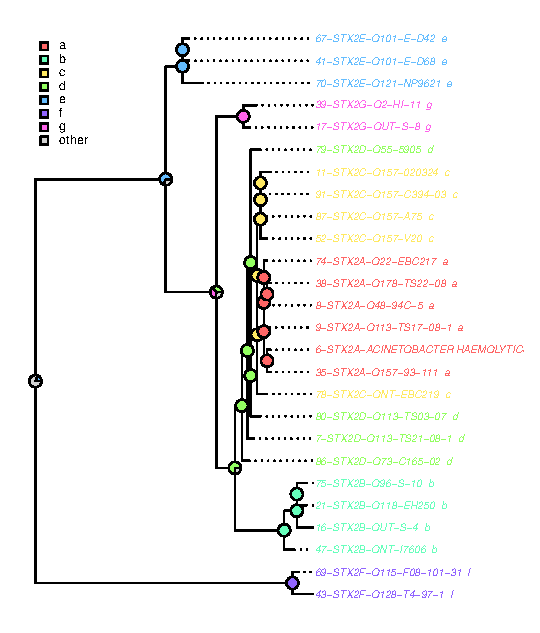
\includegraphics{fig01.eps}}
\caption{Phylogenetic tree for select Stx2 genes. 
The subtype marginal likelihood is displayed at each node as a pie chart. \DIFaddbeginFL \DIFaddFL{Subtype is indicated by color as shown in the legend. }\DIFaddendFL The full Stx2 tree is displayed in Supplementary Figure S1.}\label{fig:01}
\end{figure}

\DIFdelbegin \DIFdel{Phylotyper }\DIFdelend \DIFaddbegin \DIFadd{PPhylotyper }\DIFaddend was designed to be incorporated into a WGS workflow.  
The main input into Phylotyper is assembled genome sequences \DIFaddbegin \DIFadd{(in fasta format)}\DIFaddend .  
Putative loci needed for the subtype scheme are identified in the input genomes using BLAST \citep{Camacho2009}.
The identified loci are then sent to the Phylotyper subtype prediction module.
It is possible in Phylotyper to use multiple loci for subtype prediction.
Individual loci alignments are concatenated to form a single superalignment that is used to build the phylogenetic tree.

Currently, \DIFaddbegin \DIFadd{the Phylotyper package includes the following }\DIFaddend subtype schemes for \emph{Escherichia coli}\DIFdelbegin \DIFdel{(}\textit{\DIFdel{E. coli}}%DIFAUXCMD
\DIFdel{) are available in the Phylotyper package, and in addition to Stxinclude intimin and serotyping  }\DIFdelend \DIFaddbegin \DIFadd{: Stx, intimin and serotype O- and H-types  }\DIFaddend (Supplementary Table~1).
However, the Phylotyper software \DIFdelbegin \DIFdel{aslo }\DIFdelend \DIFaddbegin \DIFadd{also }\DIFaddend has the capability to add new subtype schemes \DIFaddbegin \DIFadd{(instructions are provided here: }\url{https://github.com/superphy/insilico-subtyping}\DIFadd{)}\DIFaddend . 
Creating a new subtype scheme will save the required reference files, allowing newly added schemes to be easily re-run from Phylotyper.
\DIFaddbegin \DIFadd{To add a new subtype scheme for use in Phylotyper, users require a training set of homologous sequences with assigned subtype whose phylogenetic grouping is predictive of the subtype.
Phylotyper assumes that the provided training sequences are 1) homologous, specifically, they are suitable for alignment and phylogenetic reconstruction 2) the sequence phylogeny is correlated with the subtype distribution and 3) the set is representative of the range of sequences that make up a subtype.
}\DIFaddend Checks are built-in to the \DIFdelbegin \DIFdel{new subtype pipeline to ensure the assumptions of the Phylotyper approach are not violated}\DIFdelend \DIFaddbegin \texttt{\DIFadd{new}} \DIFadd{pipeline to validate the submitted reference set.
Each new subtype is subject to two tests and results are reported to the user.
The first test checks that the distribution of inter-patristic phylogenetic distances between instances of the same subtype is both smaller and distinct from subtypes that are different.
This test can identify isolated cases of potentially mislabelled subtype genes that are tightly clustered with other subtypes.
A second check computes the accuracy measure, F-score, through a leave-one-out cross-validation; a procedure which uses each sequence in the training set as a test input to estimate positive and negative prediction rates (see Supplementary Methods for details).
The performance metrics: recall and F-score rapidly decrease as the correlation between the training set phylogeny and subtype distribution decreases (Supplementary Figure S2).
These checks verify that the training set sequences' phylogenetic grouping is predictive of the subtype.
There is no check that can confirm the training set covers all subtypes in a particular scheme; Phylotyper can only predict subtypes that are represented in the training set.
It is important that the user monitor schemes and update it as gaps are identified.
Phylotyper is designed to return a }\texttt{\DIFadd{non-significant/undetermined}} \DIFadd{result when encountering an unknown subtype that has no representative in the training set}\DIFaddend .

\section{Results}

\DIFdelbegin \DIFdel{To compare the performance of }\DIFdelend \DIFaddbegin \DIFadd{Phylotyper is a progression from the sequence-similarity approach that is the basis of current }\textit{\DIFadd{in silico}} \DIFadd{subtype prediction strategies.
To compare }\DIFaddend Phylotyper to a sequence similarity-based approach, we ran \DIFaddbegin \DIFadd{two validations that looked at how both methods perform when confronted with 1) gene sequence or 2) subtype class not present in the training set.
The first validation was }\DIFaddend a leave-one-out \DIFdelbegin \DIFdel{cross validation analysis.
For this assessment}\DIFdelend \DIFaddbegin \DIFadd{cross-validation test that iterated through each gene in the training set, retraining the prediction tools on a reduced training set that excludes the selected test gene, and then confirming if the retrained predictor could recover the subtype of the test gene.
This validation tests how the predictors perform when run on a distinct sequence that is not in the training set.
The second validation examined how the predictors perform when tested with a gene that has a subtype, not in the reference set.
In this validation, each subtype was iterated over and all genes that are assigned the subtype were removed from the training set.
In each iteration, we recorded the number of false-positive subtype assignments when the test sequences were used as input.
The correct response for the predictors was to return a negative result since the subtype does not exist in the training set.
For these assessments}\DIFaddend , we developed a \DIFdelbegin \DIFdel{mock }\DIFdelend sequence-similarity based tool that assigns putative subtypes using BLAST.
\DIFdelbegin \DIFdel{The leave-one-out analysis examined the four }\DIFdelend \DIFaddbegin \DIFadd{This generalized BLAST tool, based on the approach used in \mbox{%DIFAUXCMD
\citep{Joensen2015}
}%DIFAUXCMD
, assigns a query sequence a subtype when the top BLAST match from an annotated reference database is above a pre-selected percent identity and alignment coverage cutoff.
Details how the assessment was conducted are available in Supplementary methods.
The assessment examined the five }\DIFaddend subtype schemes available in Phylotyper\DIFdelbegin \DIFdel{. The results of the analysis indicated that the precision of the Phylotyper method is consistently higher than a top-BLAST hit }\DIFdelend \DIFaddbegin \DIFadd{: Stx1, Stx2, Eae, H-type (FliC), O-type (Wzy }\& \DIFadd{Wzx).
When tasked with assigning a novel gene sequence not in the training set in the leave-one-out validation, Phylotyper consistently had higher precision than a top-BLAST-hit approach.
The average precision in Phylotyper was 0.99 versus 0.96 in the top-BLAST-hit }\DIFaddend approach (Supplementary Table S2).
\DIFaddbegin \DIFadd{The BLAST approach also often had lower recall rates; it had an average recall of 0.81 compared to 0.90 with Phylotyper.
Similarly, when entire subtype classes were withheld from the training set, Phylotyper had consistently lower false positive rates for all subtypes schemes tested; the average false positive rate in this test case was 0.11, while in the BLAST approach, the average false positive rate was 0.30.
A separate assessment for the V-typer tool; a Stx subtype predictor, was run using selected Stx gene sequences from the experimentally-verified Phylotyper training set \mbox{%DIFAUXCMD
\citep{CARRILLO2016}
}%DIFAUXCMD
.
The test Stx genes had sufficient surrounding DNA sequence to support }\textit{\DIFadd{in silico}} \DIFadd{PCR.
In total, 24 Stx gene sequences were tested with the V-typer tool and V-typer returned results for 7, all correct.
Phylotyper correctly predicted the subtype for all these genes.
Based on this level of recall, it appears conditions in the Stx subtype environment are challenging for simulated PCR.
}

\DIFadd{All new or updated subtype schemes added in Phylotyper are subject to a leave-one-out cross-validation test.
The test is part of the }\texttt{\DIFadd{add}} \DIFadd{pipeline and is used to estimate the F-score of the subtype scheme. 
The F-score reflects the predictive capability of the subtype scheme. 
If the associated phylogeny for the training set gene sequences is not correlated with the subtype distribution, this will be reflected in the F-score. 
To demonstrate this property, we randomly assigned subtypes for increasing proportions of the genes in the training set and computed the F-score with the leave-one-out validation for each proportion level.
The F-score and recall rapidly decrease as the proportion of randomly altered subtypes increases (Supplementary Figure S2).
}\DIFaddend 

\section{Discussion}

From assembled WGS data, Phylotyper can assign \DIFdelbegin \DIFdel{unclassifed strains a molecular }\DIFdelend \DIFaddbegin \DIFadd{unclassified strains a }\DIFaddend subtype.
Currently\DIFaddbegin \DIFadd{, }\DIFaddend the Phylotyper software offers subtyping schemes for \textit{E. coli}.
It can, however, be applied to \DIFdelbegin \DIFdel{most molecular }\DIFdelend \DIFaddbegin \DIFadd{other }\DIFaddend subtype schemes and Phylotyper includes functionality to build new schemes.
\DIFaddbegin \DIFadd{Phylotyper can produce predicted subtypes from any input sequence that is strongly correlated with the subtype distribution, however, input sequences with a direct biological causal link to the subtype will have fewer caveats; A gene sequence that is causal cannot become disassociated from the subtype through recombination or horizontal gene transfer.
Outside of }\textit{\DIFadd{E. coli}}\DIFadd{, the PCR-based capsular typing system for }\textit{\DIFadd{Haemophilus influenzae}}\DIFadd{, Neurotoxin serotyping in }\textit{\DIFadd{Clostridium botulinum}} \DIFadd{and the haemagglutinin and neuraminidase types in Influenza A virus are all examples of potential future subtype schemes that we are incorporating into Phylotyper.
We plan on expanding the Phylotyper resource by adding and updating high-quality subtype schemes for other pathogens.
We encourage users to contact us with their new subtype schemes or updates to schemes (}\url{https://github.com/superphy/insilico-subtyping}\DIFadd{).
}\DIFaddend 

\DIFdelbegin \DIFdel{Performance testing showed that Phylotyper is more robust than an approach based solely on sequence similarity.
}\DIFdelend \DIFaddbegin \DIFadd{The main strategy currently in use by other }\textit{\DIFadd{in silico}} \DIFadd{tools for predicting subtypes is to use sequence similarity to annotated gene alleles.
Query genomes or genes are matched to alleles that are attributed the subtype phenotype or are correlated with the distribution of the subtype.
For example, SerotypeFinder uses BLAST to find the top matches based on sequence similarity to O-antigen processing genes for }\textit{\DIFadd{in silico}} \DIFadd{O-typing and the flagellin genes for H-typing }\textit{\DIFadd{E. coli}} \DIFadd{genes \mbox{%DIFAUXCMD
\citep{Jenkins2015}
}%DIFAUXCMD
.  
O-type and H-type are transferred from the top matches to the queries provided they are above coverage and percent identity thresholds.
This general strategy of allele matching is also applied in the EcOH tool \mbox{%DIFAUXCMD
\citep{Ingle2016}
}%DIFAUXCMD
, however, the EcOH tool can directly use unassembled sequence reads as input. The EcOH tool aligns reads to alleles linked to }\textit{\DIFadd{E. coli}} \DIFadd{O-types and H-types, and identifies the top candidates that have an alignment score above pre-defined thresholds.
Phylotyper is comparatively more robust as it generates fewer Type-I errors when encountering novel alleles or subtypes not present in the training set.
With the allele matching strategy, the reference set make-up can have a greater impact on performance.
When alleles or even subtypes are missing in the reference database, the sequence similarity approach more frequently generates false positive predictions.
Alternatively, }\DIFaddend Phylotyper computes an empirical model of subtype evolution to predict subtypes for unclassified sequences.
By estimating the phylogenetic distribution of each subtype, Phylotyper \DIFdelbegin \DIFdel{can more easily identify }\DIFdelend \DIFaddbegin \DIFadd{is less likely to make a Type-I error when encountering }\DIFaddend a novel subtype or \DIFdelbegin \DIFdel{accurately classify a novel sequence }\DIFdelend allele. 
The \DIFaddbegin \DIFadd{empirical testing we performed demonstrated this behavior; 
the rate of false positive classifications was significantly lower than in a sequence-similarity approach in validations where we withheld an allele or an entire subtype from the training set and used it as a test input.
V-typer takes a distinct approach; it directly simulates the }\textit{\DIFadd{in vitro}} \DIFadd{wet-lab PCR procedure used to perform Stx subtyping \mbox{%DIFAUXCMD
\citep{CARRILLO2016}
}%DIFAUXCMD
. 
V-typer's direct replication of a wet-lab method }\textit{\DIFadd{in silico}} \DIFadd{means it can only be applied to subtypes schemes that use PCR. 
Additionally, we found in our evaluation of Stx subtypes that it failed to generate predictions for most test cases.
From a methodology standpoint, Phylotyper has an additional benefit over current methods; the }\DIFaddend phylogenetic framework in Phylotyper provides a statistical likelihood for interpreting \DIFdelbegin \DIFdel{novel alleles}\DIFdelend \DIFaddbegin \DIFadd{results}\DIFaddend .
In comparison, \DIFdelbegin \DIFdel{the performance of a }\DIFdelend \DIFaddbegin \DIFadd{there is no built-in mechanism in the }\DIFaddend sequence similarity approach \DIFdelbegin \DIFdel{is highly dependent on the reference database.
This type of approach, there is no inherient mechanism to identify novel alleles }\DIFdelend \DIFaddbegin \DIFadd{to quantify the level of confidence in assigning alleles a subtype}\DIFaddend .

Subtypes are mainly used as a proxy for evolutionarily-related bacterial strain groups or to infer phenotypes.
\DIFdelbegin \DIFdel{Recent analysis of serotype data revealed several inconsistencies between molecular subtype and genomic data \mbox{%DIFAUXCMD
\citep{DebRoy2016}
}%DIFAUXCMD
.
Subtypes predicted using a phylogenetic framework is more consistent with the main uses of subtype information, so 
Phylotyper is uniquely capable to transition }\DIFdelend \DIFaddbegin \DIFadd{A recent analysis of O-antigen serotypes and their associated O-antigen gene sequences in }\textit{\DIFadd{E. coli}} \DIFadd{found that the sequence data indicated several changes to the organization of the O-groups \mbox{%DIFAUXCMD
\citep{DebRoy2016}
}%DIFAUXCMD
.
There are potentially other subtype schemes that would show discrepancies between genetic data and subtype grouping.
A tool that can evaluate the ability of a genotype to predict a subtype would be better equipped for developing the new subtype schemes or updating current schemes for WGS workflows.
Phylotyper's }\texttt{\DIFadd{add}} \DIFadd{pipeline tests subtype schemes for their predictive accuracy by returning an F-score based on a cross-validation assessment.
The validation verifies that the phylogeny generated by the training set sequences can be used to predict the subtypes with a high level of accuracy.
We showed in empirical tests that the farther a subtype is dissociated from the input gene's phylogeny, the lower the F-score computed in the Phylotyper }\texttt{\DIFadd{add}} \DIFadd{pipeline.
In addition to this subtype-level verification, Phylotyper also computes confidence scores for each individual prediction that reflect the rate of subtype change occurring at the input gene's phylogenetic locale.
If an input sequence falls in a region in the phylogenetic tree where the subtype is highly fluid due to evolution or poor subtype-genotype correlation, users would be notified in the confidence score and in the phylogenetic tree visualization output by Phylotyper. 
Phylotyper's ability to inform users about the level of agreement between the subtype assignments and genotype makes it uniquely capable of transitioning }\DIFaddend historical subtype data to new \DIFdelbegin \DIFdel{WGS }\DIFdelend \DIFaddbegin \DIFadd{whole genome sequence-based }\DIFaddend systems.\vspace*{-10pt}


\section*{Funding}

This work is funded in part by the Public Health Agency of Canada and a grant from the Genomics Research and Development Initiative\vspace*{-12pt}

\bibliographystyle{natbib}

\bibliography{phylotyper}


\end{document}
